\documentclass[12pt,a4paper]{article}
\usepackage{amsmath}
\usepackage[english]{babel}
\usepackage[latin1]{inputenc}
\setlength\topmargin{0in}
\setlength\headheight{0in}
\setlength\headsep{0in}
\setlength\textheight{10in}
\setlength\textwidth{6.5in}
\setlength\oddsidemargin{0in}
\setlength\evensidemargin{0in}
\usepackage{graphicx}


\title{Advanced Information Systems project proposal:\\
Query on structurally heterogeneous dataspaces}
\author{Sartori Enrico}
\date{A.y. 2008/2009}

\begin{document}
\maketitle
\subsection*{Project Scope}
The main aim of this project is to implement a model which can support the
execution of queries on dataspaces with different structures.
The differences I'm going to handle in this project are at a structural
level, not at a syntactic one.

The model will be able to answer queries in the form of sets of
pairs (attribute name, attribute value), the answer will be the list of
the objects which satisfies the search criteria.

The way I choose to realize this model is through the implementation of an
indexing structure, which can be used to retrieve the information needed.
The drawback of this solution is represented by the consumption of space,
needed for realize the index, but it provides higher performances in term
of time than a search through the whole dataset.


\subsection*{Index structure}
The index can be represented by a tree which contains, as nodes the
attributes of the various records and as leafs identifiers of the objects
in the dataset. Visiting the tree gives the possibility to gather the ids
of the entities which satisfy the search criteria.

This structure needs to be in main memory in order to operate, but with
large dataset is could not be always possible. It could be interesting to
implement ways to deactivate the less used branches of the tree and store
them on disk in order to limit memory consumption.

\begin{center}
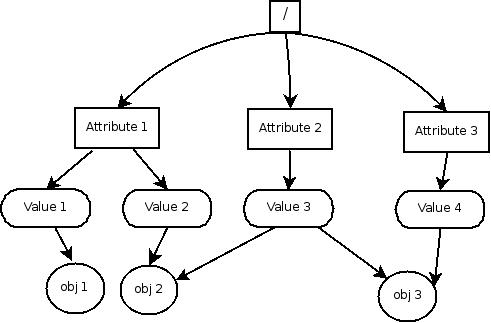
\includegraphics[scale=0.50]{tree.jpg}
\end{center}

The structure of the tree can evolve as new item are added to the dataset,
maintaining its characteristics: if a new attribute is encountered a new
node is added to the tree with its value as child. If the attribute is
already in the tree it's value is added as child of the already existing
node.

The first things which need to be implemented is, anyway, a set of
utilities used as a generator of dataspaces with the requested features
(differences in structure, but with equal attribute names). 

\end{document}
